\chapter{绪论}
\citestyle{numbers}

作为现代人工智能的最重要的分支,人工神经网络(artificial neural network, ANN)近年来获得迅速发展。学术界不断提出新的神经网络理论,算法和结构,提高网络模型的表征能力和性能,从而解决各类人工智能问题;
工业界也相继将神经网络技术应用于图像识别(image recognition)、目标检测(object detection)、语音识别(speech recognition)、自然语言处理(natural language processing, NLP)等领域。然而随着神经网络技术解决的问题越来越复杂,神经网络模型朝着规模越来越大,拓扑结构越来越复杂,层数越来越深的方向发展,因此应用神经网络技术需要庞大的存储资源,计算资源和能耗才能完成运算,这不仅给传统的处理平台如CPU和GPU带来巨大的挑战, 而且导致神经网络应用无法部署到嵌入式设备或者移动智能设备中。

研究者从软件和硬件两个方面来来试图解决这个问题。在软件方面, 近些年来,研究者利用稀疏(sparsity)、量化(quantization)、矩阵分解(matrix decomposition)、熵编码(entropy encoding)等技术缩小神经网络模型的规模,实现神经网络深度压缩;其中稀疏被证明是其中最有效的一个策略,稀疏对神经网络的拓扑结构进行裁剪,从而减少神经网络参数数量和计算量,使得稀疏神经网络能够部署到嵌入式设备中。在硬件方面,研究者提出并设计了神经网络专用加速器,从而代替CPU/GPU完成神经网络运算,减少神经网络执行时间,降低能耗。

然而,稀疏技术会使得原始稠密神经网络规则的拓扑结构转变为稀疏不规则的结构,因此使得CPU,GPU和部分加速器不能从稀疏特性中获得性能提升;尽管有部分加速器能够支持稀疏,但是效果并不理想。因此本文提出了一种软硬件结合的方法处理稀疏神经网络的不规则性,从算法和架构设计的角度提出多种优化策略,显著提升处理稀疏网络的效果。

本章首先介绍神经网络技术发展和应用。然后介绍神经网络处理平台的发展。接着介绍神经网络技术面临的挑战。最后介绍本文的主要研究内容及贡献。

\section{神经网络技术的应用}

\subsection{神经网络技术发展历程}

人工神经网络的发展和成熟已经经历了四个时期。第一个时期主要建立了单个神经元的模型和学习规则。第二个时期主要建立了单层网络的模型和学习规则。第三个时期是多层神经网络蓬勃发展的时期,神经网络开始应用到多个领域。第四个时期神经网络的理论获得长足发展,同时深度神经网络在涌现的同时被不断优化和改善,深度神经网络在图像处理、目标检测、语音识别、自然语言处理等领域有着越来越广泛的应用。

第一个时期,研究者提出单个神经元模型对应的学习规则。学术界普遍认为神经网络领域的先锋是~\citet{mcculloch1943logical},他首次正式提出了简洁又统一的神经元模型。1949年,~\citet{hebb1963organizations, gerstner2002mathematical}首次提出了生物神经网络中存储信息的单位--突触(synapse),并提出了学习过程就是修改突触的过程这一条重要的规则,这条规则是目前许多神经网络学习训练的基础。1952年,~\citet{hodgkin1952quantitative}利用动态方程建立了神经元脉冲发射的模型。1956年~\citet{taylor1956electrical}使用联想记忆神经网络(associative memory)的方法模仿了许多不同的认知模型。1958年,\citet{rosenblatt1958perceptron}提出了一套学习突触权值和神经元阈值的方法,最终完成了一个特定的信息处理任务,并提出了感知器(perceptron)的原型。

第二个时期,研究者重点研究的是单层网络的模型和学习规则。1960年,~\citet{widrow1960adaptive}采用最小二乘法(least mean-square algorithm)提出了线性适应元(adaptive linear element),这是一种自适应的模式分类神经元。FitzHugh-Nagumo神经元模型~\cite{fitzhugh1961impulses}被广泛用于模拟感官系统中生物神经元的振荡行为。它使用相空间结合霍奇金-赫克斯利方程(Hodgkin-Huxley equations)的方法将神经纤维的生理状态划分为多个区域(包括活跃,压抑,增强,休息等),形成一个生理状态图,从而帮助研究者观察多种生理现象。1967年~\citet{minsky1967computation}从自动机理论和计算理论的角度深入研究了研究了McCulloch和Pitts提出的神经元模型。1969年~\citet{minsky1969perceptron}发现了单层感知机在处理信息任务时的局限性,并提出了多层感知机,然而多层感知机的学习规则在当时并没有深入研究,因此阻碍了神经网络的发展。~\citet{cainiello1961outline}提出当神经元受到的激励处于某个阈值时,该神经元不能被激活。1972年,~\citet{nagumo1972response}在此基础上提出了一种非线性的神经元模型,当一个恒定频率的脉冲序列作用于神经元时候,由于脉冲序列的振幅随时间减少,神经元被激活的频率也会随之减少。

第三个时期,研究者开始重点研究多层神经网络的模型和学习规则。在这个时期,贝叶斯方法,高斯过程,支持向量机(support vector machine,SVM)和多层神经网络都试图与生物模型结合,从而解释大脑的认知,学习,记忆等功能。1982年,\citet{hopfield1982neural}将统计物理的概念应用于循环神经网络模型,提出了突触对称连接的神经网络,即Hopfield nets,这是80年代神经网络复兴的主要原因之一。这种简单优美的模型将记忆储存为激活值中的模式。之后,广义Hopfield网络(generalized Hopfield network,GHN)用多层神经网络代替了单层神经网络结构,该结构被不断研究和发展。~\citet{zurada1996generalized}证明GHN拥有多个稳定状态,能够保证原始Hopfield网络的稳定性。因此,各种基于GHN的网络不断被提出来解决不同的问题。1984年,~\citet{hindmarsh1984model}提出了现象学模型(phenomenological model),它能够将复杂的微分方程减少到三个,但是这个相对简单的模型能够解释合理地神经元的震荡现象。1985年,~\citet{ackley1985learning}提出了玻尔兹曼机(Bolzmann machine),它在信息理论方面有着广泛的应用。玻尔兹曼机基于模拟退火算法(simulated annealing),产生周期性的随机网络,并且根据玻尔兹曼分布模拟产生输入信号。其中,~\citet{kirkpatrick1983optimization, vcerny1985thermodynamical}提出的模拟退火算法是一个基于统计力学来解决优化问题的方法。1986年,~\citet{rumelhart1986learning}应用反向传播(back propagation,BP)算法来训练神经网络,从而解决了~\citet{minsky1969perceptron}提出的多层感知机难以进行学习的问题。由于多层前馈网络的训练经常采用BP算法,人们也常把将多层前馈网络直接称为BP网络。BP网络能学习和存贮大量的输入-输出模式映射关系,而无需事前揭示描述这种映射关系的数学方程。它的学习规则是使用最速下降法(梯度下降法),通过反向传播来不断调整网络的权值和阈值,使网络的误差平方和最小。90年代有不少研究将神经网络与概率理论相结合,从而诞生了统计机器学习方法(statistical machine learning)。\citet{mackay1992practical, bishop1995neural}将贝叶斯技术(Bayesian technique)应用于到神经网络中,用于解决推理,回归和分类等问题。同时,~\citet{williams1996gaussian}将高斯方法论(methodology of Gaussian )引入到神经网络领域。1998年,\citet{vapnik1998statistical}提出了支持向量机(SVM)。SVM的基本想法是利用kernel产生非线性表示,从而解决非线性的问题。支持向量机在模式识别,回归和密度估计等方面有着非常广泛的应用,尽管SVM被有些研究者被认为是神经网络的一个分支,但是学术界普遍认为SVM和神经网络是两个不同的领域。

第四个时期,研究者开始研究深度神经网络(deep neural network, DNN),深度神经网络由多种不同的层构成,输入数据依次通过各个层被逐层处理,最终被分类, 识别或者检测。深度神经网络还包括卷积神经网络(convolutional neural network, CNN)和循环神经网络(recurrent neural network);前者广泛应用于计算机视觉~\cite{krizhevsky2012imagenet,simonyan2014very, ren2015faster},而后者广泛应用于语音处理~\cite{hinton2012deep, amodei2015deep, ze2013statistical}或者自然语言处理~\cite{conneau2016very}。最近轰动全球的成果就是谷歌旗下的Deep Mind团队所设计的Alpha Go~\cite{moyer2016google},在围棋上先手战胜李世石和柯杰等顶级棋手。

\subsection{神经网络的应用和发展}

下面,我们将介绍神经网络在图像处理、目标检测、语音识别和自然语言处理领域的应用和发展。

\subsubsection{神经网络模型在图像分类领域的应用}
在2012年,深度神经网络在图像识别和分类领域领域取得了非常优秀的效果,~\citet{krizhevsky2012imagenet}提出的AlexNet网络结构,在ILSVRC-2012上top-5的错误率为$34.2\%$。 
AlexNet的主要结构是5个卷积层和3个全连接层,其中卷积层用于提取图像的特征,全连接层用来整合卷积层提取出的特征并进行分类。

研究者发现,深度神经网络比浅层神经网络具有更强的表征能力,拥有更高的精度。在2014年,~\citet{simonyan2014very}提出了VGG16网络,VGG16共由13个卷积层和3个全连接层,对比AlexNet的5个卷积层,能够提取出更高层次的特征。VGG16在ImageNet数据集~\cite{deng2009imagenet}上top-5的错误率为$25.3\%$。

然而网络的层数不能无限增加,网络层数过多,不仅会导致梯度消失(vanishing gradient),梯度爆炸(exploding gradient)或者过拟合(over-fitting)的问题,导致神经网络难以进行训练;还会出现网络退化的问题,
导致神经网络的表征能力下降,精度降低。因此,研究者提出了不同的网络拓扑结构,试图增加网络的层数,增加网络的表征能力。

~\citet{szegedy2015going}提出了GoogLenet网络,GoogLenet网络深度达到了22层。它最主要的特征在于使用了inception结构,从而更好地利用了网络中的计算资源,并且在不增加计算负载的情况下,增加网络的宽度和深度。inception结构的主要思想在于卷积视觉网络中一个优化的局部稀疏结构怎么样能由一系列易获得的稠密子结构来近似和覆盖。为了避免patch对齐问题,作者限制了inception结构中滤波器的大小为1x1,3x3,5x5。最终GoogleNet网络在ImageNet数据集上top-5的错误率为$26.7\%$。

~\citet{he2016deep}在2016年提出了深度残差网络(deep residual network),在ImageNet中斩获图像分类、检测、定位三项的冠军。ResNet通过shortcut的结构进行参差学习,解决了增加深度带来的退化问题,这样能够通过单纯地增加网络深度,来提高网络性能,作者在ImageNet上实验了一个152层的残差网络,比VGG深8倍,最终使得top-5错误率下降到$3.57\%$。

\subsubsection{神经网络模型在目标检测领域的应用}

\zadd{除了图像识别/分类,深度神经网络在目标检测领域也有广泛应用,并且取得了非常理想的效果。2014年,~\citet{girshick2014rich}提出了RCNN网络解决目标检测问题,RCNN的主要思想是将检测问题转化成为分类问题。
RCNN主要包括四个步骤,第一步,采用选择性搜索(selective search)对一张图像生成1K\~{}2K个候选区域(proposal region);第二步,使用深度神经网络对每一个候选区域提取特征;第三步,使用SVM分类器对提取的特征进行分类;第四步,使用回归器精细修正选框(bonding box)位置。RCNN在VOC2007上的mAP是$58\%$左右。}

RCNN存在着重复计算的问题(候选区域有几千个,多数都是互相重叠,重叠部分会被多次重复提取特征),于是~\citet{girshick2015fast}借鉴~\citet{he2014spatial}的SPP-net的思路提出了Fast-RCNN,跟RCNN最大区别就是Fast-RCNN将候选区域映射到CNN的最后一层卷积层上,这样一张图片只需要提取一次特征,大大提高了速度,也由于流程的整合以及其他原因,在VOC2007上的mAP也提高到了$68\%$。

Fast-RCNN的速度瓶颈在搜索候选区域上,于是~\citet{ren2015faster}提出了Faster-RCNN,将搜索候选区域也交给CNN来做。Fater-RCNN中的搜索候选区域网络(region proposal netwrok)实质是一个Fast-RCNN,这个Fast-RCNN输入的候选区域的是固定的(把一张图片划分成$n\times n$个区域,每个区域给出9个不同规模和比例),输出的是对输入的固定proposal是属于背景还是前景的判断和对齐位置的修正(regression)。Region proposal network的输出再输入到第二个Fast-RCNN做更精细的分类和选框的位置修正。Fater-RCNN速度更快了,而且用VGG作特征提取时在VOC2007上mAP能到$73\%$。

神经网络在目标检测领域还在持续发展,研究者不断提出新的网络和方法如Mask-RCNN~\cite{he2017mask},YOLO~\cite{redmon2016you}等来提高网络运行速度,提高网络的精度。

\subsubsection{神经网络模型在语音识别领域的应用}
\zadd{目前最好的语音识别系统采用双向长短时记忆网络(bidirectional LSTM)~\cite{graves2005framewise, graves2013speech, graves2013hybrid},这种网络能够对语音的长时相关性进行建模,从而提高识别正确率。但是双向LSTM网络存在训练复杂度高、解码时延高的问题,尤其在工业界的实时识别系统中很难应用。}

\zadd{卷积神经网络早在2012年就被用于语音识别系统~\cite{abdel2012applying},并不断被研究和改进~\cite{abdel2012applying, zhang2017towards} ,但始终没有大的突破。主要的原因是其使用固定长度的帧拼接作为输入,无法看到足够长的语音上下文信息;另外一个缺陷将CNN视作一种特征提取器,因此所用的卷积层数很少,表达能力有限。}
    
\zadd{
2017年,微软在人工智能领域取得的最新突破~\cite{xiong2017microsoft},微软语音识别系统错误率降低到$5.1\%$,准确率已经超过专业速记员。微软语音识别系统在语音模型上采用了6个不同的神经网络,并行地进行识别其中包括了应用于计算机视觉的残差网络(ResNet)和循环神经网络(RNN)。在此基础上,再用4个神经网络做语言模型,然后重新整合。所以微软语音识别系统上是10个神经网络在同时工作,最终将识别错误率降低到$5.1\%$。
}

\subsubsection{神经网络模型在自然语言处理领域的应用}
\zadd{自然语言处理无疑依然是深度学习领域有待攻克的下一个重大领域。}

\zadd{提取语义特征是NLP的一个重要话题。由于卷积神经网络(CNN)能够有效提取高层次的特征,因此CNN被应用于NLP领域。~\citet{kim2014convolutional}使用CNN应用于各种句子的分类任务,包括情绪、主体性和问题类型分类,并且获得了非常理想的结果。~\citet{denil2014modelling}在此基础上,提出了动态卷积神经网络(dynamic CNN)进行语义建模。随后,~\citet{yih2014semantic}引入了多列CNN(multi-column CNN)从多个方面来分析和理解知识库中问题和条目之间的语义相关性。
}

\zadd{循环神经网络能够在某种程度上“记忆”先前的计算结果和使用这些信息进行当前处理,这种特性非常适合进行自然语言处理。循环神经网络又可以分为时间递归神经网络(recurrent neural network)和结构递归神经网络(recursive neural network)。时间递归神经网络被广泛用来自然语言处理中的解决词分类(word-level classification)~\cite{lample2016neural, graves2013generating, sundermeyer2015feedforward},句子分类(sentence-level classification)~\cite{wang2015predicting, lowe2015ubuntu}和自然生成语言(natural language generation)的任务~\cite{vinyals2015neural, li2016persona}。结构递归神经网络(recursive neural network)也被应用于语义分析~\cite{socher2011parsing}。}

\zadd{除了卷积神经网络和循环神经网络,最近涌现出其他的深度学习方法来进行自然语言处理,如深度增强学习(deep reinforcement learning)~\cite{ranzato2015sequence, li2016deep},深度无监督学习(deep unsupervised learning)~\cite{kiros2015skip, dai2015semi},记忆增强网络(memory-augmented network)~\cite{kumar2016ask, sukhbaatar2015end}等。}

%\subsubsection{神经网络模型的低能耗优化技术}
%随着神经网络的应用越来越广泛,神经网络的规模不断扩大,层数不断加深,因此未来的大规模网络很难部署到嵌入式系统中。很多研究人员致力于减少神经网络的参数规模,从而减少对存储资源,计算资源和带宽的需求,加快神经网络运行速度,降低神经网络的能耗。研究者提出了许多方法来解决这个问题,主要可以分为低精度计算和裁剪技术。
%
%低精度计算主要将神经元的权值或神经元进行低比特量化,从而降低网络存储需求和运算能耗。低精度量化包括16比特定点量化~\cite{gupta2015deep},8比特量化~\cite{dettmers20158},二元权值量化~\cite{courbariaux2015binaryconnect},三元权值量化~\cite{rastegari2016xnor},2的幂次等形式的量化~\cite{zhou2017incremental};在对神经网络参数量化过程中,可能会降低网络的精度,尤其是需要注意两个情况:第一,当采用极低比特量化神经网络时,可能导致精度损失;第二,当对神经网络的权值和神经元同时进行量化时,可能导致精度损失。
%
%神经网络的裁剪技术采用剪枝直接减少神经网络中参数数量。剪枝技术~\cite{reed1993pruning, lecun1989optimal, miche2010op, han2015learning, guo2016dynamic}能够修剪神经网络中不必要的连接。如果神经元或者权值满足某些条件,那么这些神经元/权值将会被修剪,从而降低网络的复杂性,最终能够在不影响精度的情况下获得具有良好泛化性能的精简神经网络。值得注意的是,对神经网络进行裁剪会破坏稠密网络规则的拓扑结构,引入不规则性。
%
%除了上述的两种方法,研究者还采用矩阵分解,例如利用矩阵因式分解~\cite{denton2014exploiting, lebedev2014speeding}的对权值矩阵或者卷积核进行分解,在保持模型规则计算的情况下,实现神经网络压缩和加速。

\section{神经网络计算平台发展}

主流的神经网络计算平台是通用处理器,即CPU和GPU。然而CPU的性能并不能满足实际的需求,而GPU的的能耗过高。因此研究者开始为神经网络算法设计专用的加速器,使得神经网络算法在加速器上既能够满足高性能的需求,又能够满足低能耗的需求。目前有两个流行的加速平台,分别是可编程逻辑门阵列(field-programmable gate array,FPGA)和专用集成电路(application specific integrated circuit , ASIC)。

\subsection{通用处理器CPU和GPU}
CPU~\cite{chakradhar2010dynamically, vanhoucke2011improving}和GPU~\cite{farabet2009cnp, scherer2010accelerating, ciresan2011flexible, coates2013deep}是两个完成神经网络运算的通用平台。同时,在CPU和GPU上,有许多针对神经网络的高级编程框架,如Caffe~\cite{jia2014caffe},Tensorflow~\cite{abadi2016tensorflow},MXNet~\cite{chen2015mxnet},使得用户能够方便地将神经网络算法部署到CPU和GPU上进行计算。

\citet{vanhoucke2011improving}在CPU上采用多种策略对神经网络算法进行优化,包括循环展开,使用SIMD指令并行累加,调整数据保证内存对齐,使用8比特量化减少内存占用等,最终获得了4倍的性能提升。

CPU集群更能够满足大规模网络应用的性能需求。谷歌提出了由数万个CPU组成的神经网络训练框架——DistBelief~\cite{dean2012large},并用它来训练由数十亿个参数构成神经网络,训练数据集为1000万张$200\times 200$的图片,训练时间长达3天,最终在ImageNet数据集上获得了$15.8\%$的错误率。

在CPU集群中,由于核之间的通信延迟高,带宽低,因此核之间的通信会成为整个系统的瓶颈。GPU采用完全不同的体系结构,它采用单任务多数据(single program multiple data, SPMD)框架,兼有分布式存储和共享内存的优点,具有非常高的并行性。因此,GPU对于计算密集(compute intensive)型应用,如CNN和DNN,具有非常高的加速效果,性能完全超过CPU。2004年,~\citet{oh2004gpu}成功地将神经网络部署到GPU进行运算。2010年,~\citet{scherer2010accelerating}使用CUDA框架将大规模CNN部署到GPU,在训练过程中,每一个block负责一个batch运算,每一个thread负责一个权值的运算,同时利用共享内存重用输入数据或错误信号,从而大大提高内存利用率。
更进一步的,不少研究者开始全面探究如何使用GPU加速机器学习算法。

然而,CPU和GPU在处理神经网络时的效率并不高,因为这些通用处理器首先考虑的是通用性和普遍性,许多处理逻辑(包括计算和存储)对神经网络计算的支持并不理想。从计算的角度考虑,通用处理器只支持基本的计算,复杂的算术运算是通过一系列的基本计算组成,因此寄存器和内存之间需要进行频繁的数据交换,这不仅降低性能,还会带来大量的能耗。从存储的角度考虑,通用处理器采用冯·诺依曼体系中的层次化存储结构,缓存容量通常小于其他专用处理器,例如NVIDIA K20的片上缓存只有$1.5MB$,Intel E78880L的片上缓存不超过$50MB$。然而,随着神经网络的迅猛发展,神经网络的参数朝着十亿~\cite{le2013building}甚至百亿~\cite{coates2013deep}发展。有限的片上缓存($100KB$\~{}$10MB$)与超大规模的网络参数($100MB$\~{}$10GB$)之间的矛盾会导致频繁的片上缓存与片外存储之间的数据交换,进一步降低处理器性能,增加能耗开销。

\subsection{FPGA}
FPGA能够为计算密集型的应用(如CNN、DNN等)提供大量的逻辑资源,包括计算资源和存储资源。FPGA的可编程性和可重构特性允许用户自定义设计,同时能够在很短时间内完成设计评估,从而缩短开发周期,节约开发费用。尽管FPGA的性能和能效都比不上ASIC,但是研究人员仍然可以选择用FPGA代替ASIC设计神经网络加速器。

2009年,\citet{farabet2009cnp}在Xilinx Virtex-4 SX35平台上设计了一个卷积神经网络处理核,它采用多个DSP并行计算多个输出神经元的部分和。但是由于FPGA资源的限制,系统只能够运行二维卷积运算,因此无法利用不同卷积核之间的并行性。

随后在2011年,~\citet{farabet2011neuflow}在Xilinx Virtex 6平台上设计了基于可扩展的数据流的架构Neuflow,并且获得了100倍的加速比。Neuflow包含多个tile,每一个tile集成了多个一维卷积运算单元和乘加器(multiply-add accumulation, MAC),从而完成二维卷积运算;多个tile可以并行执行二维卷积运算从而完成三维卷积运算。

\citet{gokhale2014240}在Xilinx ZC706平台上设计了nn-X。这是一个可扩展的,低功耗的协处理器,主要用来加速深度神经网络。nn-X协处理器由8个运算单元组成,每个运算单元集成了一个卷积运算单元,池化运算单元和非线性运算单元;运算单元通过4通道的DMA与片外DDR3内存进行互联。nn-X的理论峰值能够达到$227GOP/s$,实际吞吐率为$200GOP/s$;整个设计的功耗为$8W$,其中核心计算模块的功耗为$4W$。

\citet{zhang2015optimizing}在VC707板卡上实现了一个吞吐量为$61.62GFLOPS$的CNN加速器,工作频率为$100MHz$。作者采用loop tiling对计算进行划分,并采用roofline model定量分析计算资源与带宽需求,从而获得最佳配置方案。~\citet{suda2016throughput}在~\citet{zhang2015optimizing}的基础上进一步进行研究,他们提出了一个基于FPGA资源约束的系统设计空间搜索(design space exploration)方案,最大化CNN加速器在FPGA上的性能。

\citet{qiu2016going}在Xilinx Zynq ZC706板卡上实现了一个CNN加速器,在$150MHz$的频率下性能为$137GOP/S$。作者对全连接层的权值进行奇异值分解(Singular Value Decomposition, SVD),从而减少内存访问,同时采用动态精度量化的方法对神经网络参数进行量化,从而减少参数存储量,进一步减少逻辑资源和能耗。

除了CNN网络,FPGA还能够加速其他类型的网络。~\citet{rice2009scaling}在FPGA上实现了分层贝叶斯网络模型,对比于的Cray XD1平台上的纯软件实现能够获得75倍。~\citet{kim2009highly}在FPGA上实现了深度信念网络模型,对比CPU实现能够获得24 \~{} 30倍的加速比。

\zadd{Microsoft提出了一项开创性计划,Project Catapult~\cite{putnam2014reconfigurable}。该计划将FPGA部署到大规模数据中心中,旨在大范围提高数据中心负载性能和能源效率,并且目前已经应用于人工智能领域。实验显示,Project Catapult能够在保持吞吐量的情况下,减少$29\%$的尾延迟(tail latency)。
}

\subsection{ASIC}
ASIC是设计师自定义功能的定制电路,相比于CPU,GPU和FPGA,它具有体积小,功耗低,可靠性高,性能高等优点。

CNN这类有高度并行性的计算密集型应用适合部署到ASIC上,因此早期的研究主要集中在如何设计加速器来快速实现卷积操作以满足实时处理的需求。
~\citet{lee1987parallel}提出了一个能够完成任意规模二维卷积运算的架构,其中处理单元采用二维网格结构互相连接。~\citet{stearns1988reconfigurable}提出了L64240的过滤器,计算单元的规模为$8\times 8$,工作频率为$20MHz$。~\citet{kamp1990programmable}提出了一个可编程的规模为$7\times 7$二维卷积核结构,工作频率为$20MHz$,内部缓存区的每一行最多能够存储512个像素。~\citet{hecht1991advanced}设计了脉动阵列的架构完成二维卷积运算。更进一步的,~\citet{lee2006super}提出了一个超级脉动阵列的结构完成二维卷积运算,其中阵列单元的输入输出带宽仅仅为1比特,能够在没有性能损失的情况下减少$2/3$的面积。

\begin{table}[h]
\centering
\caption{DianNao Family详细参数}
\footnotesize
\label{tab:diannao_family}
\begin{tabular}{lll@{~~~}llll@{~}llll@{~}lll@{~~}llll@lllll}
\toprule
accelerator & techonology($nm$) 	&area($mm^2$)   &power($nm$)    &throughput($GOP/S$)	& Application\\
\midrule
DianNao	    & ~~~~~65               &3.02			&0.485		    &~~~~452 	            & neural network\\
DaDianNao 	& ~~~~~28	            &67.73			&15.97		    &~~~~5584	            & neural network\\
PuDianNao   & ~~~~~65 	            &3.51			&0.596		    &~~~~1056	            & machine learning\\
ShiDianNao  & ~~~~~65	            &4.86			&0.320		    &~~~~194	            & CNN\\
\bottomrule
\end{tabular}
\end{table}

DianNao Family~\cite{chen2016diannao}是一系列的神经网络加速器,包括DianNao~\cite{chen2014diannao}, DaDianNao~\cite{chen2014diannao}, PuDianNao~\cite{liu2015pudiannao}和ShiDianNao~\cite{du2015shidiannao} 。我们在表~\ref{tab:diannao_family}列出了它们的详细参数。DianNao是加速器家族的第一个成员,它能够完成通用的神经网络运算,如CNN、DNN等。DaDianNao是DianNao的多核版本,它采用eDRAM作为片上缓存尽可能将神经网络的参数存储到片上,从而避免高额的片外访存开销。PuDianNao是机器学习处理器,它除了能够完成神经网络运算,还支持KNN,K-Means等多种机器学习算法。ShiDianNao是面向嵌入式设备的卷积神经网络处理器,它采用脉动阵列的形式完成神经网络的卷积运算,从而提高数据复用,减少访存能耗,实现端到端的神经网络应用。

\zadd{谷歌提出了张量处理器(tensor processing unit,TPU)~\cite{jouppi2017tpu},主要用来加速器其第二代人工智能系统Tensorflow的运行。TPU的核心是一个$256\times 256$,即65536个8位矩阵乘单元阵列(matrix multiply unit),并采用脉动阵列的形式完成神经网络运算,峰值计算能力为$92TOPS$,相比于K80有15倍的性能提升。
}
    

除了DianNao系列神经网络加速器和谷歌的TPU,最近还涌现出越来越多的加速器,如~\citet{farabet2011neuflow}提出了Neuflow,~\citet{chen2016eyeriss}提出了Eyeriss等,它们均采用脉动阵列的形式完成神经网络的运算。


\section{神经网络技术面临的挑战和目前的解决方法}

\subsection{面临的挑战}
\zadd{随着神经网络的应用越来越广泛,神经网络模型的拓扑结果越来越复杂,规模不断扩大,层数不断加深,因此未来的大规模网络很难部署到嵌入式系统中。神经网络模型的规模不断扩大,主要体现在两个方面:第一个方面,神经网络的参数(包括神经元和权值)不断增多,例如,AlexNet的网络规模超过$200MB$,VGG16的网络规模超过$500MB$;第二方面,神经网络的层数不断加深,例如ResNet网络的层数可以到达上百层甚至上千层。大规模神经网络对存储,带宽和计算提出了很高的需求,因而难以部署到嵌入式设备中。
}

\zadd{第一个问题是存储容量的问题。由于嵌入式设备或者移动设备的存储容量有限,尽管在手机端本地运行深度神经网络能够减少网络带宽,进行任务实时处理,获得更好的隐私保护,但是这些大规模的神经网络需要耗费巨大的存储开销,因此阻碍了深度神经网络应用被部署到移动应用程序。
}

\zadd{第二个问题是能耗问题。大型神经网络需要大量的带宽加载神经网络数据(包括拓扑结构,输入,神经元,权值等),同时需要大量的计算资源完成神经网络的运算,这个过程需要耗费巨大的能量。考虑到移动设备电池容量的限制,高能耗的应用,如深层神经网络应用将难以部署。能源消耗主要来源于访存能耗。在$45nm$工艺下,一个32位浮点加法需要消耗$0.9pJ$的能量,一次32位SRAM缓存访问耗费$5pJ$的能量,而一次32位DRAM内存访问需要$640pJ$的能量,这个能耗几乎是浮点加法操作的3个数量级。大型神经网络无法缓存在片上的SRAM中,因此需要需要在片外的DRAM与片上的SRAM之间频繁进行数据交换,从而产生巨大的访存能耗开销。例如我们以$20fps$运行一个拥有10亿个连接的神经网络,那么需要为DRAM访存提供至少$P = (20Hz)\times (640pJ)\times (1G) = 12.8W$的功率,已经完全超过了大多数手机电池能够提供的功率。
}

\subsection{目前的解决方法}
\zadd{为了应对这些挑战,研究者从各个方向做出了各种各样的努力,包括算法级 (例如Drop out~\cite{srivastava2014dropout}、Sparsity~\cite{han2015learning}),架构级 (例如短位宽运算~\cite{holi1993finite}甚至是1比特运算~\cite{rastegari2016xnor},非精确计算~\cite{venkataramani2014axnn})和物理级(例如,动态电压调整技术~\cite{pillai2001real})。其中,剪枝(pruning)技术是目前解决这个问题最有效的方法之一。}


\begin{figure}[ht]
\centering
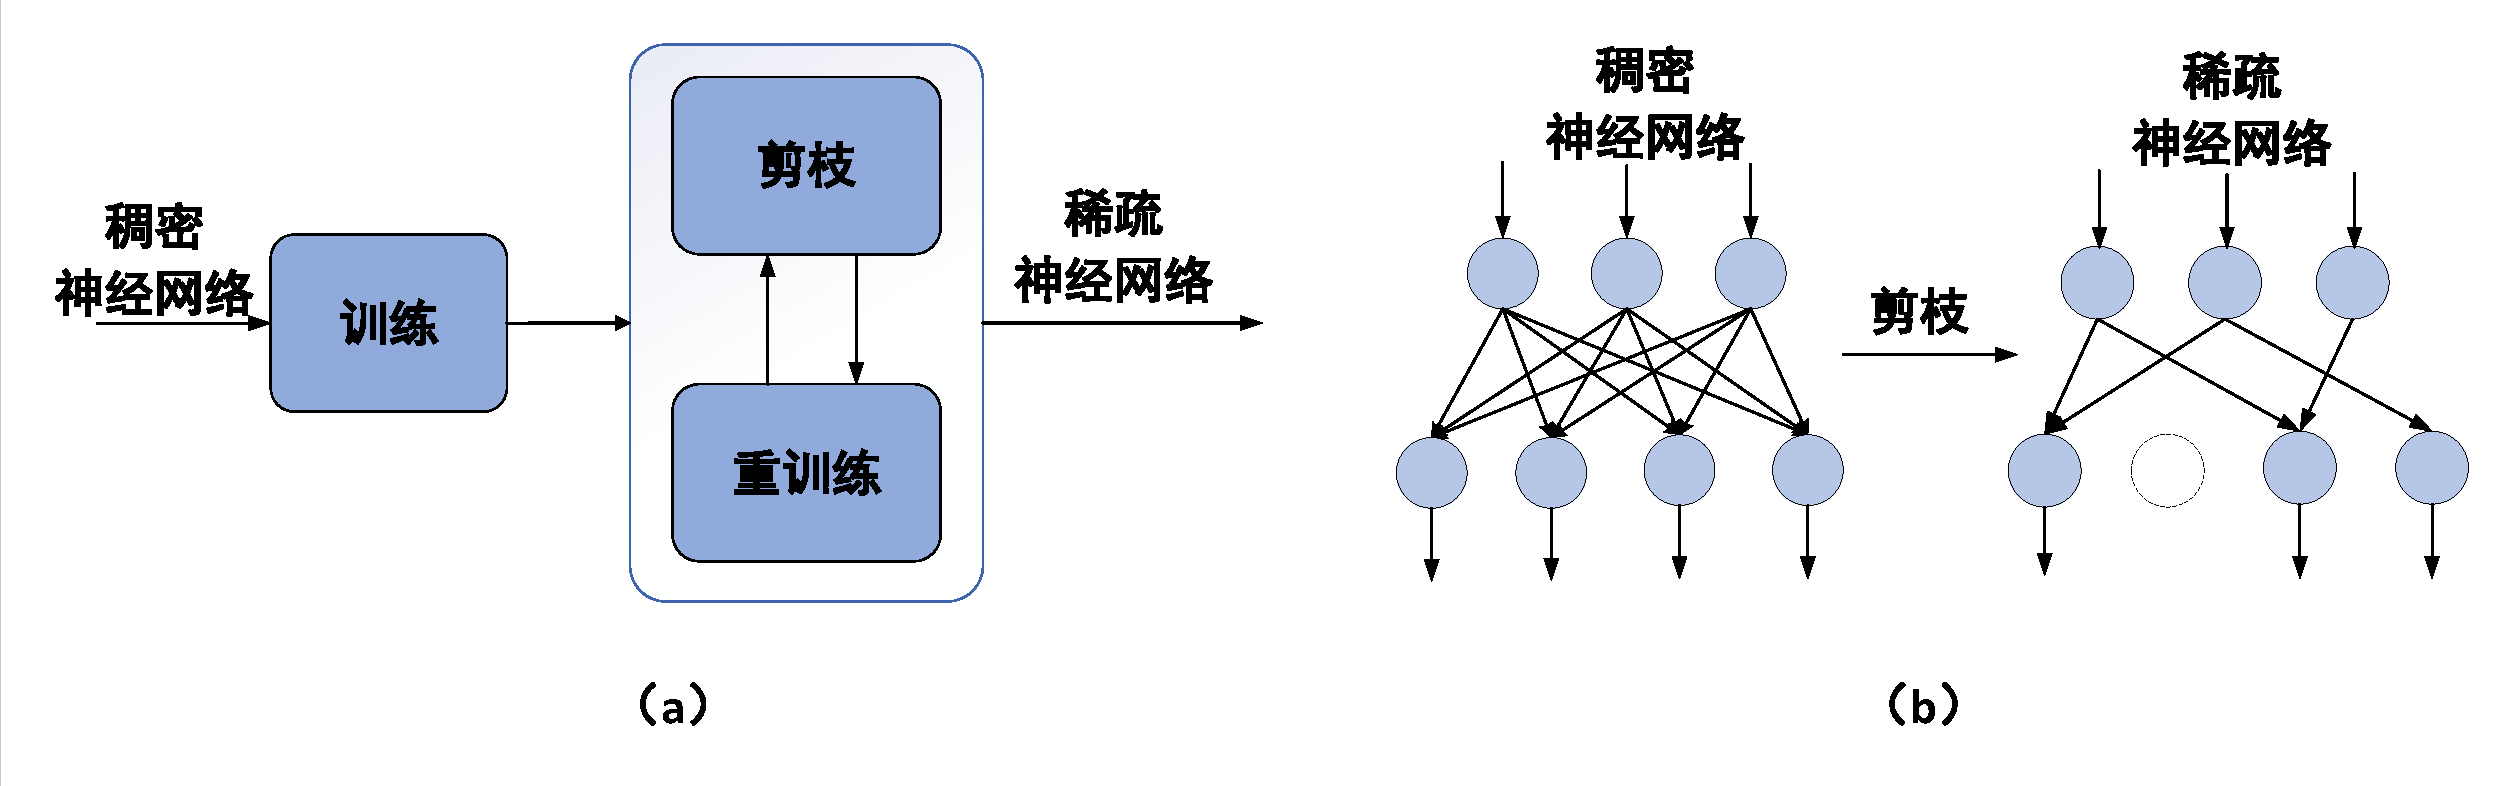
\includegraphics[width=1.0\columnwidth]{pruning.pdf}
\caption{\footnotesize (a)剪枝流程  (b)剪枝前后神经网络}
\label{fig:pruning}
\end{figure}

\zadd{
神经网络的剪枝技术通过裁剪神经元或者突触接减少神经网络中参数规模。剪枝技术~\cite{reed1993pruning, lecun1989optimal, miche2010op, han2015learning, guo2016dynamic}能够修剪神经网络中不必要的连接。如果神经元或者权值满足某些条件,那么这些神经元/权值将会被修剪,从而降低网络的复杂性,最终能够在不影响精度的情况下获得具有良好泛化性能的精简神经网络。图~\ref{fig:pruning}(a)和(b)分别是剪枝的流程和剪枝前后的神经网络~\cite{han2015learning}。
}

\subsection{稀疏神经网络的不规则性}

\zadd{尽管稀疏神经网络能够在理论上减少计算量,存储量和数据传输量,但是稀疏技术会引入\textbf{不规则性(irregularity)},即导致原本规则的神经网络拓扑结构转变为不规则的形式,从而使得规则计算模式转变为不规则。目前的处理平台由于存在诸多问题,无法有效地处理不规则的稀疏神经网络。根据~\cite{zhang2016cambricon},CPU和GPU并不能很好地支持稀疏神经网络运算,即使使用稀疏矩阵运算库,如sparseBLAS或者cuBLAS,也不能取得非常理想的加速效果,在某些情况下处理稀疏网络的性能甚至比处理稠密神经网络的性能还要差。例如,CPU平台上,除了 LeNet-5 网络,稀疏的AlexNet网络和VGG16网络的性能都比稠密网络差,性能平均降低了2.11 倍。在GPU平台上,运行稀疏神经网络仅仅能提高$23.34\%$的性能,对比于稀疏神经网络高达$90.84\%$的稀疏度,这个性能提升是非常有限的。因此通用的CPU和GPU并不能利用稀疏的特性。
}

\begin{table}[h]
\footnotesize
\centering
\caption{现有支持稀疏的神经网络加速器的比较}
\label{tab:comp}
\begin{tabular}{@{}lllll@{}llllllll}
  \toprule
  ~& 权值稀疏 & 神经元稀疏 & 注释\\
  \midrule
  Eyeriss~\cite{chen2017eyeriss} & \ding{55} & \ding{52} & 只能跳过计算,无法带来性能提升 \\
  Cambircon-X~\cite{zhang2016cambricon} & \ding{52} & \ding{55} &\\
  Cnvlutin~\cite{albericio2016cnvlutin} &\ding{55} & \ding{52}&\\
  EIE~\cite{han2016eie} &\ding{52}& \ding{52}& 只适合全连接层\\ 
  ESE~\cite{han2017ese} &\ding{52}& \ding{55}& 只适合稀疏的LSTM层\\
  SCNN~\cite{angshuman2017scnn} &\ding{52}& \ding{52}& 需要额外计算部分和的坐标,全连接层效果不理想\\
\bottomrule
\end{tabular}
\end{table}

\zadd{尽管目前有不少支持稀疏神经网络的加速器~\cite{chen2017eyeriss, zhang2016cambricon, albericio2016cnvlutin, han2016eie, han2017ese, angshuman2017scnn},但是它们仍然不能有效地处理稀疏神经网络带来的\textbf{不规则性}。它们不但需要显著的处理稀疏的成本,而且不能完全支持所有稀疏类型。例如Cambricon-X~\cite{zhang2016cambricon}中支持稀疏的逻辑占总面积的$31.07\%$,占功耗的$34.83\%$,而且只能支持权值稀疏。Cnvlutin~\cite{albericio2016cnvlutin}只能利用神经元稀疏。EIE~\cite{han2016eie}虽然能够同时利用权值和神经元稀疏,但是它只能适用于稀疏的全连接层,不能运行稀疏卷积层。SCNN~\cite{angshuman2017scnn}能够在卷积层同时利用神经元和权值稀疏,但是对全连接层的支持并不理想,同时会引入复杂的坐标计算过程。
}


\section{主要研究内容及贡献}

\begin{figure}[ht]
\centering
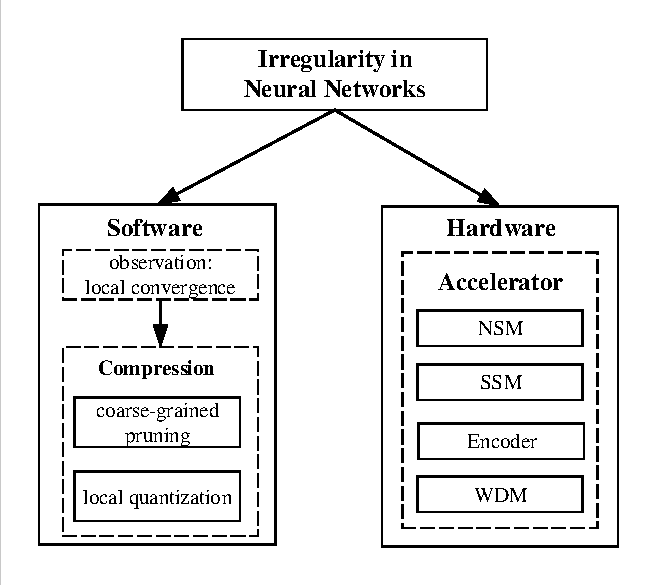
\includegraphics[width=0.8\columnwidth]{idea.pdf}
\caption{本文主要研究内容和创新点}
\label{fig:idea}
\end{figure}

最近的研究~\cite{han2015learning,han2015deep,wang2016cnnpack,zhou2017incremental}表明,神经网络可以在保持精度的前提下,通过稀疏,量化,低精度等方式进行深度压缩,从而减少参数存储量,计算量和访存量。然而,稀疏技术会使得原本规则的神经网络计算变得不规则,因此CPU,GPU以及一些不支持稀疏的加速器并不能从中受益。尽管,最近出现了一些能够支持稀疏的神经网络加速器~\cite{chen2017eyeriss,zhang2016cambricon,albericio2016cnvlutin,han2016eie,han2017ese,angshuman2017scnn},但是挖掘稀疏的效果并不理想,利用稀疏的效率也不高。

本文提出了一种软硬件结合方法(software/hardware cooprative approach)来处理稀疏神经网络的不规则性。我们首先提出了粗粒度剪枝算法,从而减少稀疏神经网络的不规则性,同时我们结合局部量化和熵编码对神经网络进行深度压缩。然后我们设计了粗粒度稀疏神经网络加速器Cambricon-S,来处理粗细度稀疏的神经网络,新型加速器有高性能和和低能耗的特点。本文的主要贡献如图~\ref{fig:idea}所示,可以归纳如下:

1.本文首次提出采用软硬件结合的方法处理稀疏神经网络不规则性。在软件方面我们提出了一种新的压缩算法对神经网络进行深度压缩,压缩算法中包含的粗粒度稀疏算法能够减少稀疏神经网络的不规则性;在硬件方面,我们提出了粗粒度稀疏神经网络加速器来Cambricon-S高效处理粗粒度稀疏,从而获得性能提升,同时降低能耗。

2. 本文观察到了局部收敛(local convergence)的现象,即在训练过程中,神经网络的权值不是一种随机分布的情况,大的权值会聚集成簇,我们通过大量实验证明局部收敛的现象出现在许多的神经网络中。本文根据观察到的局部收敛现象,提出了一种新的神经网络压缩算法。压缩算法包括三个步骤,分别是粗粒度剪枝(coarse-grained pruning),局部量化(local quantization)和熵编码(entropy coding)。粗粒度剪枝将神经网络的权值分为多个权值块,当一个权值块符合某个条件时将从网络拓扑中被完全剪除,粗粒度稀疏的神经网络对比与细粒度稀疏的神经网络拥有更低的不规则度。局部量化将权值分为多个子区域,然后在每一个子区域内分别进行量化,进一步压缩神经网络。之后,我们采用熵编码对神经网络进行无损压缩。

3. 本文设计并提出了首个能够支持粗粒度稀疏神经网络的加速器微结构。该微结构不仅能够处理普通的稠密神经网络,还能够通过打开/关闭稀疏处理模块支持多种稀疏/量化情况,包括神经元稀疏,粗粒度权值稀疏,神经元/权值同时稀疏,局部量化等。新型加速器能够非常高效的利用稀疏和量化,获得非常理想的性能和能耗。

4. 本文针对神经网络加速器的计算特性,设计了专用的性能模拟器。该模拟器能够高速,精准地模拟神经网络在加速器上运行的性能。

\section{论文的组织结构}
本文第一章介绍了本文的工作背景。我们主要从神经网络技术和神经网络加速器两方面介绍神经网络的发展简史,基本原理和面临的问题,在此基础上,我们提出了本文的主要研究内容和创新点。

第二章介绍了神经网络相关的背景知识。首先我们介绍了神经网络模型,对神经网络的多种不同类型的层计算进行详细分析。然后我们介绍了神经网络的低能耗技术,包括低精度计算技术和裁剪技术。最后我们介绍最新神经网络加速器的相关工作,其中我们重点介绍了稀疏神经网络加速器。

第三章提出了一种新的神经网络压缩方法。首先我们观察到神经网络的权值在训练过程中有局部收敛的现象,即大的权值容易聚集成簇。基于局部收敛,我们提出了粗粒度剪枝的策略,将多个权值同时进行裁剪操作;然后我们提出局部量化的方案进一步利用局部收敛,减少表示权值的比特数,进一步对神经网络进行压缩;最后我们利用熵编码对神经网络进行无损压缩。大量实验证明:新的压缩方法能够对神经网络进行深度压缩,同时减少稀疏神经网络的不规则性。

第四章提出了一个粗粒度稀疏神经网络加速器,能够快速处理经过深度压缩的神经网络。首先,我们观察粗粒度稀疏神经网络的特点,提出了设计加速器的三个原则。然后我们根据这三个设计原则,提出了新型加速器的架构,新的加速器能够充分利用神经元稀疏,粗粒度权值稀疏和局部量化,从而提高性能,降低功耗。最后我们为新型加速器设计了专用的编程框架,减轻用户的编程负担。

第五章提出了一个新型加速器专用的性能模拟器,我们根据新型加速器的特性,设计了一个性能优化的模拟器代替周期精确模拟器,从而在误差允许的范围内,快速完成对加速器的性能评估。

第六章,我们对加速器进行详细的性能和能耗评估,在七个benchmark上,我们将Cambricon-S与CPU,GPU,DianNao和Cambricon-X进行性能和能耗的比较。最后我们根据实验结果详细分析了新型加速器能够获得高性能和低能耗的原因。

最后一章我们对本文进行总结,并展望了未来的研究工作。
